\documentclass[11pt, fleqn]{article}

\usepackage{amsmath}
\usepackage{amssymb}
\usepackage{amsthm}
\usepackage{mathtools}
\usepackage{hyperref}
\usepackage{ulem}
\usepackage{enumitem}
\usepackage[left=0.75in, right=0.75in, bottom=0.75in]{geometry}
% \usepackage{float}
\usepackage{floatrow}
\usepackage{graphicx}
\usepackage[export]{adjustbox}

\usepackage{sectsty}
\sectionfont{\centering}

\usepackage[perpage]{footmisc}

\usepackage{fancyhdr}
\pagestyle{fancy}
\fancyhf{}
\lhead{190100044 \& 190100055}
\rhead{CS 215: Assignment 5}
\renewcommand{\footrulewidth}{1.0pt}
\cfoot{Page \thepage}

\setlength{\parindent}{0em}
\renewcommand{\arraystretch}{2}%

\title{Assignment 5: CS 215}
\author{
\begin{tabular}{|c|c|}
     \hline
     Devansh Jain & Harshit Varma \\
     \hline
     190100044 & 190100055 \\
     \hline
\end{tabular}
}
\date{\today}

\begin{document}

\maketitle

\renewcommand{\arraystretch}{1}

\section*{Question 2}
\addcontentsline{toc}{section}{Question 2}
\setcounter{equation}{0}
\setcounter{figure}{0}

\subsection*{Instructions for running the code}
\begin{enumerate}[itemsep=-1ex]
    \item Unzip, \texttt{cd} into \texttt{q2/code}, open and run \texttt{q2.m}
    \item The respective plots for MLE and PME will be created and saved to \texttt{q2/results/}
\end{enumerate}

First, we draw data samples $\{x_i\}_{i=1}^N$ from the $X \thicksim U(0,1)$. \\
Then, we generate $\{y_i\}_{i=1}^N$ by applying strictly monotonic transformation function $f(y) = (-1/\lambda) log(x)$. \\
\begin{equation*}
    \begin{aligned}
        p_X(x) &= 1 \hspace{1em} \text{if } x \in (0,1) \\
            &= 0 \hspace{1em} \text{(otherwise)} \\
        p_Y(y) &= p_X(f^{-1}(y)) \bigg| \frac{d}{dy} f^{-1}(y) \bigg| \\
        f^{-1} (y) &= e^{-\lambda y} \\
        p_Y(y) &= |\lambda| e^{-\lambda y} \hspace{1em} \text{if } y \in (0,\infty) \\
            &= 0 \hspace{3em} \text{(otherwise)}
    \end{aligned}
\end{equation*}

We are given that $\lambda = 5$. We generate samples accordingly but for calculation of MLE we are not given any constraints on $\lambda$, except that it can not be zero.

Likelihood function is $L(\{y_i\}_{i=1}^N|\lambda) = |\lambda|^N \  exp(-\lambda \sum_{i=1}^N y_i)$. \\
Gamma prior function, given, is $Q_\Lambda(\lambda;\alpha,\beta) = \frac{\beta^{\alpha}}{\Gamma(\alpha)} \lambda^{\alpha-1} e^{-\beta\lambda} = \frac{\beta}{\Gamma(\alpha)} (\beta\lambda)^{\alpha-1} e^{-\beta\lambda} $ \\
\begin{equation*}
    \begin{aligned}
        log L(\{y_i\}_{i=1}^N|\lambda) &= N log |\lambda| - \lambda \sum_{i=1}^N y_i \\
        \frac{\partial}{\partial \lambda} log L(\{y_i\}_{i=1}^N|\lambda) \bigg|_{\lambda = \hat{\lambda}} & = \frac{N}{\hat{\lambda}} - \sum_{i=1}^N y_i \\
        \text{ML estimate of $\lambda$},\ \hat{\lambda} &= \frac{N}{\sum_{i=1}^N y_i}  
    \end{aligned}
\end{equation*}

As the prior function is non-zero only for non-zero $\lambda$, for calculating Posterior mean we can use $|\lambda| = \lambda$,

\begin{equation*}
    \begin{aligned}
        \text{Posterior pdf } P(\lambda|\{y_i\}_{i=1}^N) &= P(\{y_i\}_{i=1}^N|\lambda) P(\lambda) / P(\{y_i\}_{i=1}^N) \\
        P(\{y_i\}_{i=1}^N) &= \int_{\lambda=0}^{\infty} P(\{y_i\}_{i=1}^N|\lambda) P(\lambda) d\lambda
    \end{aligned}
\end{equation*}

\begin{equation*}
    \begin{aligned}
        \text{Posterior mean } &= E \bigg[ P(\{y_i\}_{i=1}^N|\lambda) P(\lambda) / P(\{y_i\}_{i=1}^N) \bigg] \\
            &= \frac{\int_{\lambda=0}^{\infty} \lambda P(\{y_i\}_{i=1}^N|\lambda) P(\lambda) d\lambda}{\int_{\lambda=0}^{\infty} P(\{y_i\}_{i=1}^N|\lambda) P(\lambda) d\lambda}
    \end{aligned}
\end{equation*}


\begin{equation*}
    \begin{aligned}
        P(\{y_i\}_{i=1}^N|\lambda) P(\lambda) &= \bigg( \lambda^N \  e^{-\lambda \sum_{i=1}^N y_i} \bigg) \bigg( \frac{\beta}{\Gamma(\alpha)} (\beta\lambda)^{\alpha-1} e^{-\beta\lambda} \bigg) \\
            &= \frac{1}{\beta^{N-1} \Gamma(\lambda)}\  (\beta\lambda)^{N+\alpha-1}\ exp(-\lambda (\beta + \sum_{i=1}^N y_i)) \\
            &= \frac{1}{\beta^{N-1} \Gamma(\lambda)}\ (\lambda(\beta + \sum_{i=1}^N y_i))^{N+\alpha-1} \bigg(\frac{\beta}{\beta + \sum_{i=1}^N y_i}\bigg)^{N+\alpha-1}\ exp(-\lambda (\beta + \sum_{i=1}^N y_i)) \\
            &= \frac{\beta^\alpha}{(\beta + \sum_{i=1}^N y_i)^{N+\alpha-1} \Gamma(\lambda)} \bigg( (\lambda (\beta + \sum_{i=1}^N y_i))^{N+\alpha-1}\ exp(- (\lambda (\beta + \sum_{i=1}^N y_i))) \bigg) \\
        \lambda P(\{y_i\}_{i=1}^N|\lambda) P(\lambda) &= \frac{\beta^\alpha}{(\beta + \sum_{i=1}^N y_i)^{N+\alpha} \Gamma(\lambda)} \bigg( (\lambda (\beta + \sum_{i=1}^N y_i))^{N+\alpha}\ exp(- (\lambda (\beta + \sum_{i=1}^N y_i))) \bigg) \\
    \end{aligned}
\end{equation*}

Using the fact that $\int_{t=0}^\infty t^x \exp(-x) dt = \Gamma(x)$ and $\Gamma(x+1)/\Gamma(x) = x$,

\begin{equation*}
    \begin{aligned}
        \int_{\lambda=0}^\infty P(\{y_i\}_{i=1}^N|\lambda) P(\lambda) &= \frac{\beta^\alpha}{(\beta + \sum_{i=1}^N y_i)^{N+\alpha-1} \Gamma(\lambda)} \Gamma(N+\alpha-1) \\
        \int_{\lambda=0}^\infty \lambda P(\{y_i\}_{i=1}^N|\lambda) P(\lambda) &= \frac{\beta^\alpha}{(\beta + \sum_{i=1}^N y_i)^{N+\alpha} \Gamma(\lambda)} \Gamma(N+\alpha) \\
        \text{Posterior mean } &= \frac{\int_{\lambda=0}^{\infty} \lambda P(\{y_i\}_{i=1}^N|\lambda) P(\lambda) d\lambda}{\int_{\lambda=0}^{\infty} P(\{y_i\}_{i=1}^N|\lambda) P(\lambda) d\lambda} \\
            &= \frac{\Gamma(N+\alpha)}{\Gamma(N+\alpha-1)(\beta + \sum_{i=1}^N y_i)} \\
            &= \frac{N+\alpha-1}{\beta + \sum_{i=1}^N y_i}
    \end{aligned}
\end{equation*}

Given, $\alpha = 5.5,\ \beta = 1$, $\hat{\lambda^{PM}} = (N+4.5) / (1+\sum y_i)$

\begin{figure}[H]
    \centering
    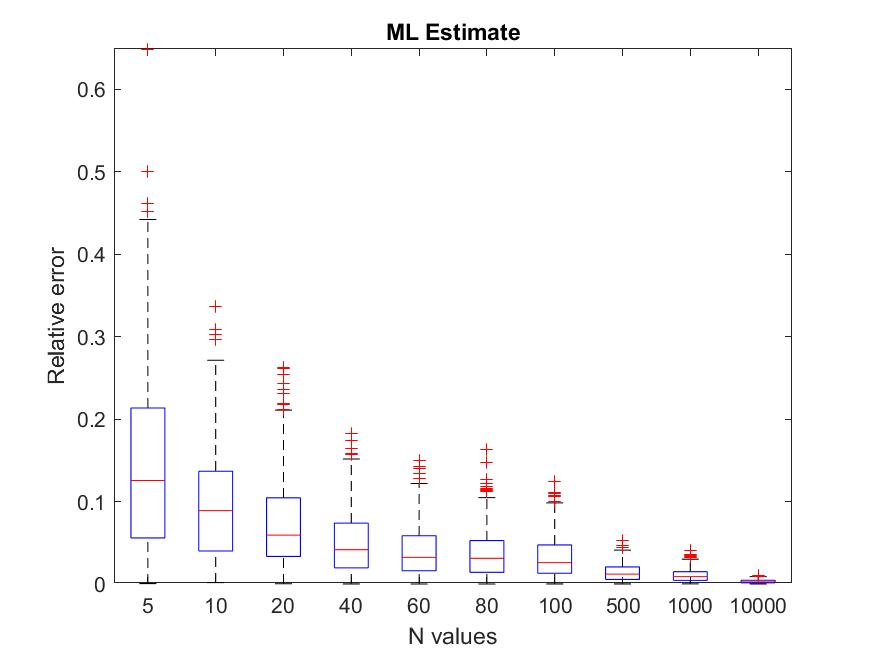
\includegraphics[scale=0.35]{q2/mle.jpg}
    \caption{ML Estimate relative error}
\end{figure}

\begin{figure}[H]
    \centering
    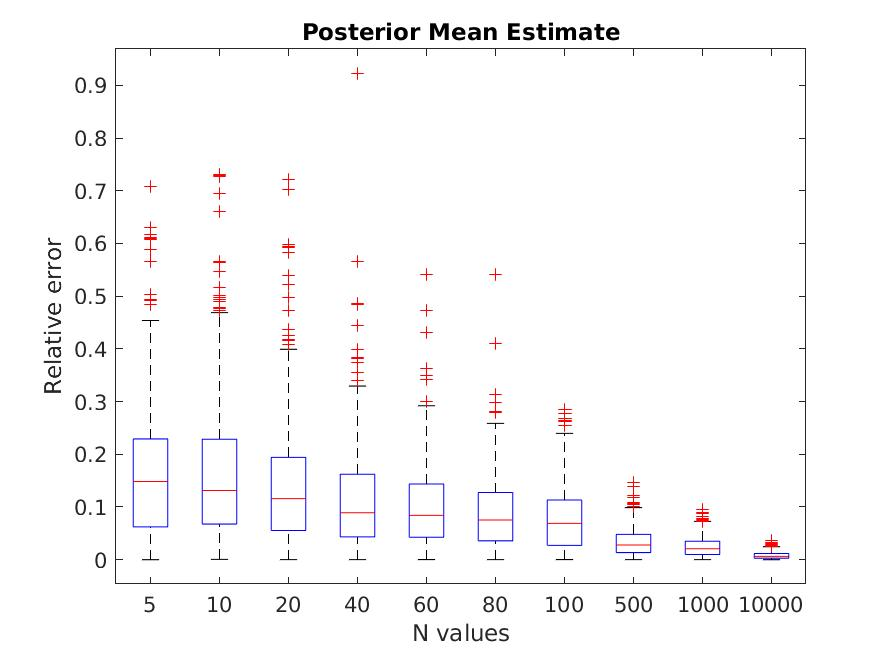
\includegraphics[scale=0.35]{q2/pme.jpg}
    \caption{PM Estimate relative error}
\end{figure}

From the formula derived for Posterior Mean Estimate, we can see that it tends to Maximum Likelihood Estimate as N tends to infinity. \\
As N increases, we also see that relative error of both Estimators tend to zero, i.e., the estimates tend towards the true value. \\
Comparing the two estimate we can see (from the plots) that Posterior Mean Estimate has less relative error than MLE (especially for small N), and thus is preferred. \\
The reason being that we use a ``prior" information about the more probable location of $\lambda$, which is close to the true value as Mode of the Prior function is at $\lambda = (\alpha - 1)/\beta = 4.5$ and Mean is at $\lambda = \alpha/\beta = 5.5$.

\end{document}
